\begin{table}[htbp]\centering\small
\setlength{\tabcolsep}{4pt}
\caption{Primary Abalone application, $n=4177,p=8$, local family. P, M8, E8, E64, U-H and H-box have finite-sample guarantees under the stated IID sampling model; M-C and M-B use asymptotic multiplier calibration. Bounds in this table are from the same full degree-pair path-LP projection. Exact enumeration (main text, Section~\ref{sec:sharp}) further sharpens several E64 endpoints, including the Height degree from $[1,3]$ to $[1,2]$, and raises the number of hub exclusions from four to five.}\label{tab:abalone}
\begin{lrbox}{\resultsbox}\begin{tabular}{lrrrrrrr}
\toprule
Test & Orders & Forced & Fixed degrees & Hubs & $W_d$ minor & $W_d$ path & $W_r$\\
\midrule
P & 104 & 0 & 1 & 0 & 3.250 & 2.625 & 6.750\\
M8 & 89 & 0 & 0 & 0 & 4.250 & 3.250 & 7.000\\
E8 & 109 & 3 & 1 & 0 & 2.125 & 1.875 & 6.500\\
E64 & 111 & 3 & 2 & 0 & 1.875 & 1.375 & 5.625\\
U-H & 42 & 0 & 0 & 0 & 6.000 & 5.500 & 7.000\\
H-box & 45 & 0 & 0 & 0 & 6.000 & 5.250 & 7.000\\
M-C & 152 & 6 & 6 & 1 & 0.250 & 0.250 & 3.250\\
M-B & 125 & 4 & 3 & 1 & 0.875 & 0.750 & 4.875\\
\bottomrule\end{tabular}\end{lrbox}\ifdim\wd\resultsbox>\linewidth\resizebox{\linewidth}{!}{\usebox{\resultsbox}}\else\usebox{\resultsbox}\fi\end{table}
For the single-matching exact reference, path projection reduces mean degree width from 3.250 to 2.625 (19.2\%). Ring count has degree [1,1] and rank [3,8], excluding hub status under the stated model. Whole weight appears as the unique sample hub in all 499 ordinary Kendall bootstrap trees, but its one-matching exact rank remains [1,8]. The multiplier-contrast projection instead gives whole-weight degree [4,4] and rank [1,1]. This nominal bootstrap declaration and the exact confidence output are reported separately.
The estimated Pearson and Kendall Abalone trees share 5 of seven edges. Both weight definitions and all edge frequencies are archived. Their agreement in this dataset does not make the population targets interchangeable outside models with a common monotone correlation ordering. Pooled and sex-stratified results, every complete-family comparison, and all Dry Bean stress outputs are supplied without selecting favorable strata.
The exact E64 construction gives whole-weight degree [3,5] and rank [1,3], excluding 4 of the eight vertices from hub status. Its mean degree width is 1.375, 47.6\% below the single-matching exact result after the same projection. It retains a finite-sample guarantee under the same sampling model; unique-hub identification and a top-three rank restriction are distinct conclusions.
\begin{figure}[!ht]\centering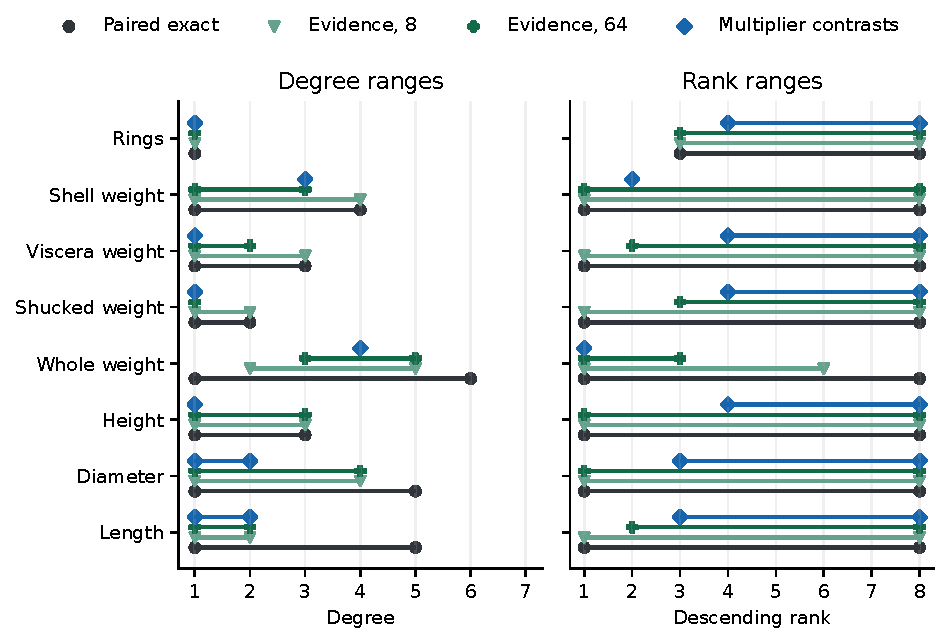
\includegraphics[width=\textwidth]{Fig_cross_section.pdf}
\caption{Degree and rank ranges for eight Abalone measurements under the four displayed calibrations, after identical path projection. P, E8 and E64 have finite-sample guarantees under the stated IID model; M-C has asymptotic multiplier calibration. Population degree ties retain their full rank ranges.}\label{fig:cross}\end{figure}
